% Created by tikzDevice version 0.12.6 on 2025-01-17 13:26:48
% !TEX encoding = UTF-8 Unicode
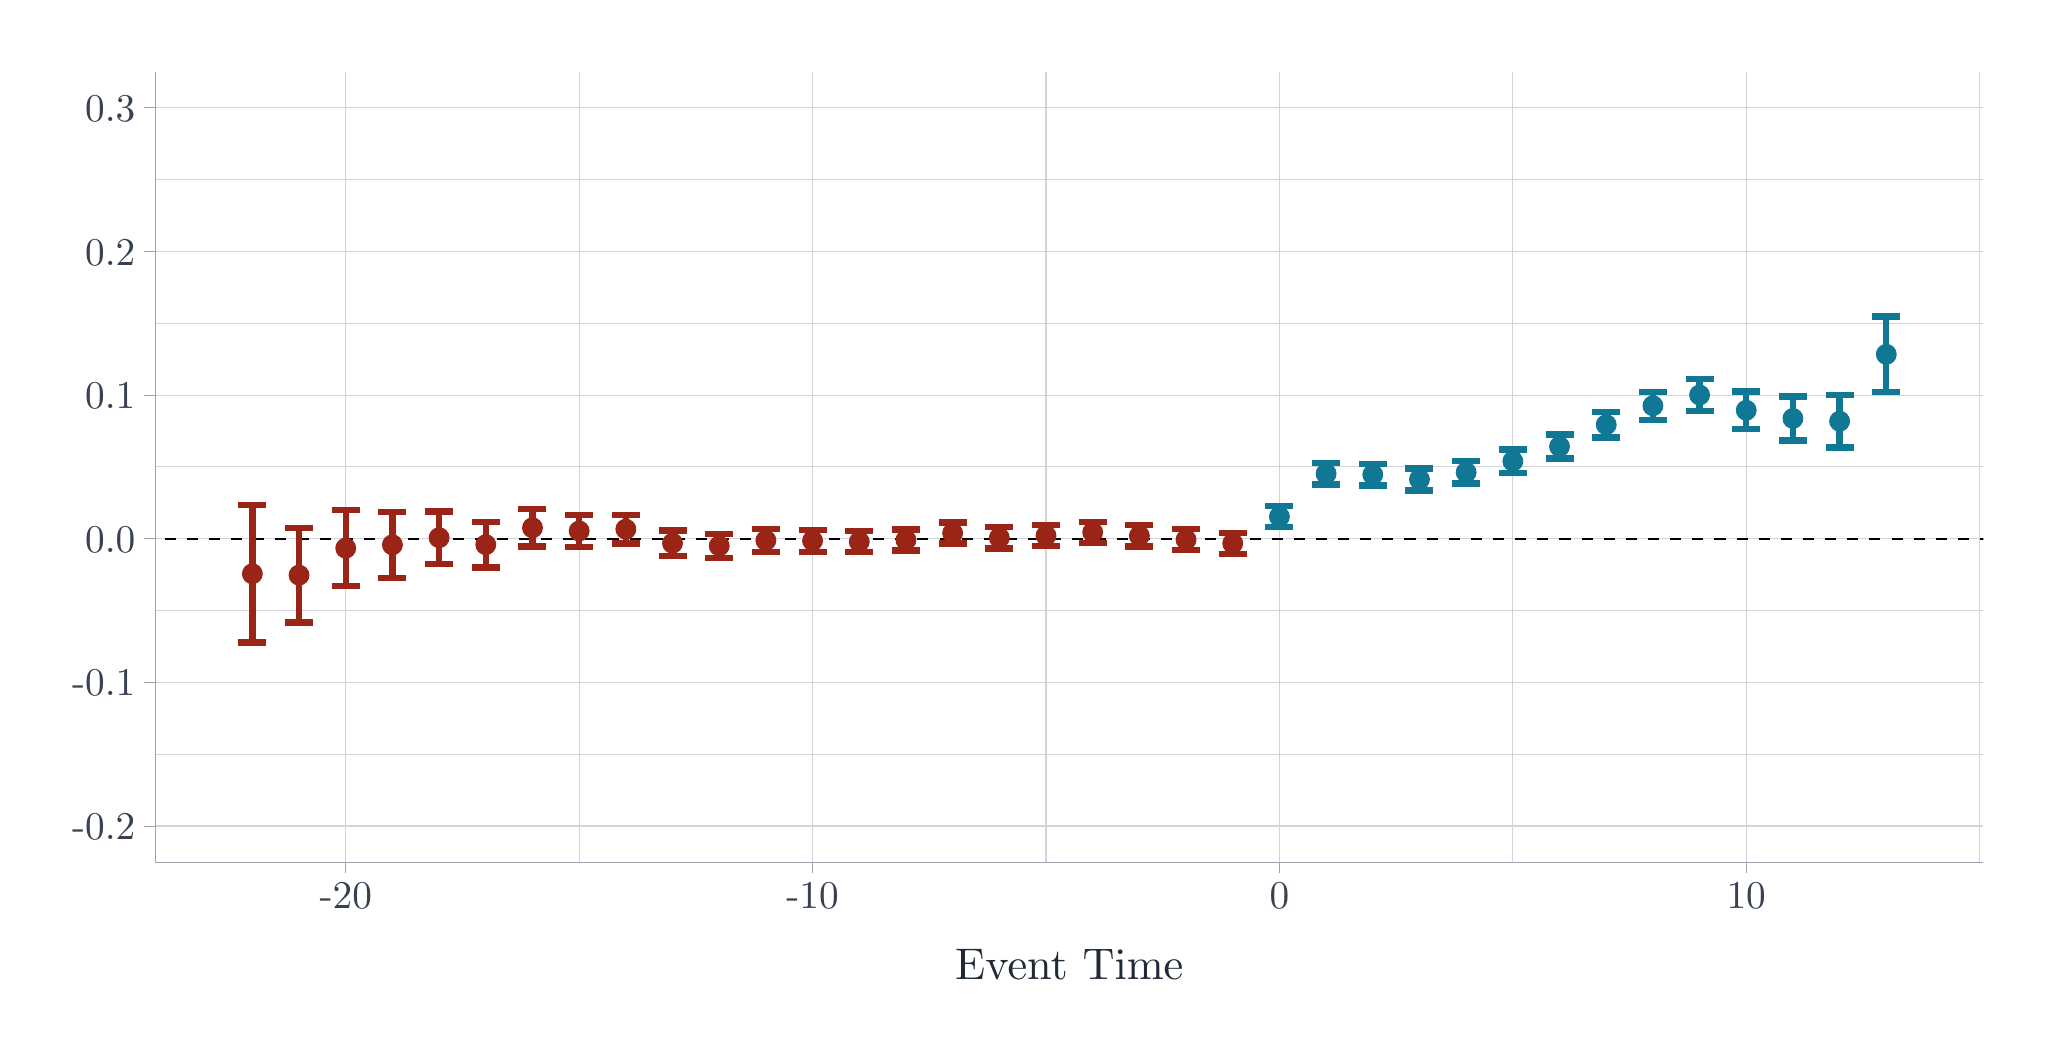
\begin{tikzpicture}[x=1pt,y=1pt]
\definecolor{fillColor}{RGB}{255,255,255}
\path[use as bounding box,fill=fillColor] (0,0) rectangle (722.70,361.35);
\begin{scope}
\path[clip] (  0.00,  0.00) rectangle (722.70,361.35);
\definecolor{drawColor}{RGB}{255,255,255}

\path[draw=drawColor,line width= 0.8pt,line join=round,line cap=round,fill=fillColor] (  0.00,  0.00) rectangle (722.70,361.35);
\end{scope}
\begin{scope}
\path[clip] ( 46.10, 59.89) rectangle (706.70,345.35);
\definecolor{drawColor}{RGB}{255,255,255}
\definecolor{fillColor}{RGB}{255,255,255}

\path[draw=drawColor,line width= 0.8pt,line join=round,line cap=round,fill=fillColor] ( 46.10, 59.89) rectangle (706.70,345.35);
\definecolor{drawColor}{RGB}{209,213,219}

\path[draw=drawColor,line width= 0.4pt,line join=round] ( 46.10, 98.81) --
	(706.70, 98.81);

\path[draw=drawColor,line width= 0.4pt,line join=round] ( 46.10,150.72) --
	(706.70,150.72);

\path[draw=drawColor,line width= 0.4pt,line join=round] ( 46.10,202.62) --
	(706.70,202.62);

\path[draw=drawColor,line width= 0.4pt,line join=round] ( 46.10,254.52) --
	(706.70,254.52);

\path[draw=drawColor,line width= 0.4pt,line join=round] ( 46.10,306.42) --
	(706.70,306.42);

\path[draw=drawColor,line width= 0.4pt,line join=round] (199.28, 59.89) --
	(199.28,345.35);

\path[draw=drawColor,line width= 0.4pt,line join=round] (367.97, 59.89) --
	(367.97,345.35);

\path[draw=drawColor,line width= 0.4pt,line join=round] (536.66, 59.89) --
	(536.66,345.35);

\path[draw=drawColor,line width= 0.4pt,line join=round] (705.35, 59.89) --
	(705.35,345.35);

\path[draw=drawColor,line width= 0.4pt,line join=round] ( 46.10, 72.86) --
	(706.70, 72.86);

\path[draw=drawColor,line width= 0.4pt,line join=round] ( 46.10,124.77) --
	(706.70,124.77);

\path[draw=drawColor,line width= 0.4pt,line join=round] ( 46.10,176.67) --
	(706.70,176.67);

\path[draw=drawColor,line width= 0.4pt,line join=round] ( 46.10,228.57) --
	(706.70,228.57);

\path[draw=drawColor,line width= 0.4pt,line join=round] ( 46.10,280.47) --
	(706.70,280.47);

\path[draw=drawColor,line width= 0.4pt,line join=round] ( 46.10,332.37) --
	(706.70,332.37);

\path[draw=drawColor,line width= 0.4pt,line join=round] (114.93, 59.89) --
	(114.93,345.35);

\path[draw=drawColor,line width= 0.4pt,line join=round] (283.62, 59.89) --
	(283.62,345.35);

\path[draw=drawColor,line width= 0.4pt,line join=round] (452.31, 59.89) --
	(452.31,345.35);

\path[draw=drawColor,line width= 0.4pt,line join=round] (621.00, 59.89) --
	(621.00,345.35);
\definecolor{drawColor}{RGB}{0,0,0}

\path[draw=drawColor,line width= 0.9pt,dash pattern=on 4pt off 4pt ,line join=round] (-614.49,176.67) -- (1367.30,176.67);
\definecolor{drawColor}{RGB}{154,36,21}
\definecolor{fillColor}{RGB}{154,36,21}

\path[draw=drawColor,line width= 0.4pt,line join=round,line cap=round,fill=fillColor] ( 81.19,164.01) circle (  3.57);

\path[draw=drawColor,line width= 0.4pt,line join=round,line cap=round,fill=fillColor] ( 98.06,163.53) circle (  3.57);

\path[draw=drawColor,line width= 0.4pt,line join=round,line cap=round,fill=fillColor] (114.93,173.27) circle (  3.57);

\path[draw=drawColor,line width= 0.4pt,line join=round,line cap=round,fill=fillColor] (131.80,174.48) circle (  3.57);

\path[draw=drawColor,line width= 0.4pt,line join=round,line cap=round,fill=fillColor] (148.67,177.05) circle (  3.57);

\path[draw=drawColor,line width= 0.4pt,line join=round,line cap=round,fill=fillColor] (165.54,174.53) circle (  3.57);

\path[draw=drawColor,line width= 0.4pt,line join=round,line cap=round,fill=fillColor] (182.41,180.62) circle (  3.57);

\path[draw=drawColor,line width= 0.4pt,line join=round,line cap=round,fill=fillColor] (199.28,179.48) circle (  3.57);

\path[draw=drawColor,line width= 0.4pt,line join=round,line cap=round,fill=fillColor] (216.15,180.14) circle (  3.57);

\path[draw=drawColor,line width= 0.4pt,line join=round,line cap=round,fill=fillColor] (233.01,175.05) circle (  3.57);

\path[draw=drawColor,line width= 0.4pt,line join=round,line cap=round,fill=fillColor] (249.88,174.09) circle (  3.57);

\path[draw=drawColor,line width= 0.4pt,line join=round,line cap=round,fill=fillColor] (266.75,176.07) circle (  3.57);

\path[draw=drawColor,line width= 0.4pt,line join=round,line cap=round,fill=fillColor] (283.62,175.96) circle (  3.57);

\path[draw=drawColor,line width= 0.4pt,line join=round,line cap=round,fill=fillColor] (300.49,175.59) circle (  3.57);

\path[draw=drawColor,line width= 0.4pt,line join=round,line cap=round,fill=fillColor] (317.36,176.23) circle (  3.57);

\path[draw=drawColor,line width= 0.4pt,line join=round,line cap=round,fill=fillColor] (334.23,178.73) circle (  3.57);

\path[draw=drawColor,line width= 0.4pt,line join=round,line cap=round,fill=fillColor] (351.10,177.01) circle (  3.57);

\path[draw=drawColor,line width= 0.4pt,line join=round,line cap=round,fill=fillColor] (367.97,177.80) circle (  3.57);

\path[draw=drawColor,line width= 0.4pt,line join=round,line cap=round,fill=fillColor] (384.84,179.00) circle (  3.57);

\path[draw=drawColor,line width= 0.4pt,line join=round,line cap=round,fill=fillColor] (401.71,177.74) circle (  3.57);

\path[draw=drawColor,line width= 0.4pt,line join=round,line cap=round,fill=fillColor] (418.58,176.32) circle (  3.57);

\path[draw=drawColor,line width= 0.4pt,line join=round,line cap=round,fill=fillColor] (435.44,175.02) circle (  3.57);
\definecolor{drawColor}{RGB}{16,120,149}
\definecolor{fillColor}{RGB}{16,120,149}

\path[draw=drawColor,line width= 0.4pt,line join=round,line cap=round,fill=fillColor] (452.31,184.63) circle (  3.57);

\path[draw=drawColor,line width= 0.4pt,line join=round,line cap=round,fill=fillColor] (469.18,200.18) circle (  3.57);

\path[draw=drawColor,line width= 0.4pt,line join=round,line cap=round,fill=fillColor] (486.05,199.85) circle (  3.57);

\path[draw=drawColor,line width= 0.4pt,line join=round,line cap=round,fill=fillColor] (502.92,198.14) circle (  3.57);

\path[draw=drawColor,line width= 0.4pt,line join=round,line cap=round,fill=fillColor] (519.79,200.66) circle (  3.57);

\path[draw=drawColor,line width= 0.4pt,line join=round,line cap=round,fill=fillColor] (536.66,204.70) circle (  3.57);

\path[draw=drawColor,line width= 0.4pt,line join=round,line cap=round,fill=fillColor] (553.53,209.99) circle (  3.57);

\path[draw=drawColor,line width= 0.4pt,line join=round,line cap=round,fill=fillColor] (570.40,217.88) circle (  3.57);

\path[draw=drawColor,line width= 0.4pt,line join=round,line cap=round,fill=fillColor] (587.27,224.72) circle (  3.57);

\path[draw=drawColor,line width= 0.4pt,line join=round,line cap=round,fill=fillColor] (604.14,228.62) circle (  3.57);

\path[draw=drawColor,line width= 0.4pt,line join=round,line cap=round,fill=fillColor] (621.00,223.10) circle (  3.57);

\path[draw=drawColor,line width= 0.4pt,line join=round,line cap=round,fill=fillColor] (637.87,220.14) circle (  3.57);

\path[draw=drawColor,line width= 0.4pt,line join=round,line cap=round,fill=fillColor] (654.74,219.15) circle (  3.57);

\path[draw=drawColor,line width= 0.4pt,line join=round,line cap=round,fill=fillColor] (671.61,243.31) circle (  3.57);
\definecolor{drawColor}{RGB}{154,36,21}

\path[draw=drawColor,line width= 2.3pt,line join=round] ( 76.13,188.80) --
	( 86.25,188.80);

\path[draw=drawColor,line width= 2.3pt,line join=round] ( 81.19,188.80) --
	( 81.19,139.22);

\path[draw=drawColor,line width= 2.3pt,line join=round] ( 76.13,139.22) --
	( 86.25,139.22);

\path[draw=drawColor,line width= 2.3pt,line join=round] ( 93.00,180.66) --
	(103.12,180.66);

\path[draw=drawColor,line width= 2.3pt,line join=round] ( 98.06,180.66) --
	( 98.06,146.40);

\path[draw=drawColor,line width= 2.3pt,line join=round] ( 93.00,146.40) --
	(103.12,146.40);

\path[draw=drawColor,line width= 2.3pt,line join=round] (109.87,186.95) --
	(119.99,186.95);

\path[draw=drawColor,line width= 2.3pt,line join=round] (114.93,186.95) --
	(114.93,159.60);

\path[draw=drawColor,line width= 2.3pt,line join=round] (109.87,159.60) --
	(119.99,159.60);

\path[draw=drawColor,line width= 2.3pt,line join=round] (126.74,186.39) --
	(136.86,186.39);

\path[draw=drawColor,line width= 2.3pt,line join=round] (131.80,186.39) --
	(131.80,162.57);

\path[draw=drawColor,line width= 2.3pt,line join=round] (126.74,162.57) --
	(136.86,162.57);

\path[draw=drawColor,line width= 2.3pt,line join=round] (143.61,186.51) --
	(153.73,186.51);

\path[draw=drawColor,line width= 2.3pt,line join=round] (148.67,186.51) --
	(148.67,167.58);

\path[draw=drawColor,line width= 2.3pt,line join=round] (143.61,167.58) --
	(153.73,167.58);

\path[draw=drawColor,line width= 2.3pt,line join=round] (160.48,182.77) --
	(170.60,182.77);

\path[draw=drawColor,line width= 2.3pt,line join=round] (165.54,182.77) --
	(165.54,166.28);

\path[draw=drawColor,line width= 2.3pt,line join=round] (160.48,166.28) --
	(170.60,166.28);

\path[draw=drawColor,line width= 2.3pt,line join=round] (177.35,187.33) --
	(187.47,187.33);

\path[draw=drawColor,line width= 2.3pt,line join=round] (182.41,187.33) --
	(182.41,173.92);

\path[draw=drawColor,line width= 2.3pt,line join=round] (177.35,173.92) --
	(187.47,173.92);

\path[draw=drawColor,line width= 2.3pt,line join=round] (194.22,185.35) --
	(204.34,185.35);

\path[draw=drawColor,line width= 2.3pt,line join=round] (199.28,185.35) --
	(199.28,173.62);

\path[draw=drawColor,line width= 2.3pt,line join=round] (194.22,173.62) --
	(204.34,173.62);

\path[draw=drawColor,line width= 2.3pt,line join=round] (211.08,185.28) --
	(221.21,185.28);

\path[draw=drawColor,line width= 2.3pt,line join=round] (216.15,185.28) --
	(216.15,174.99);

\path[draw=drawColor,line width= 2.3pt,line join=round] (211.08,174.99) --
	(221.21,174.99);

\path[draw=drawColor,line width= 2.3pt,line join=round] (227.95,179.67) --
	(238.08,179.67);

\path[draw=drawColor,line width= 2.3pt,line join=round] (233.01,179.67) --
	(233.01,170.44);

\path[draw=drawColor,line width= 2.3pt,line join=round] (227.95,170.44) --
	(238.08,170.44);

\path[draw=drawColor,line width= 2.3pt,line join=round] (244.82,178.43) --
	(254.94,178.43);

\path[draw=drawColor,line width= 2.3pt,line join=round] (249.88,178.43) --
	(249.88,169.74);

\path[draw=drawColor,line width= 2.3pt,line join=round] (244.82,169.74) --
	(254.94,169.74);

\path[draw=drawColor,line width= 2.3pt,line join=round] (261.69,180.24) --
	(271.81,180.24);

\path[draw=drawColor,line width= 2.3pt,line join=round] (266.75,180.24) --
	(266.75,171.91);

\path[draw=drawColor,line width= 2.3pt,line join=round] (261.69,171.91) --
	(271.81,171.91);

\path[draw=drawColor,line width= 2.3pt,line join=round] (278.56,179.93) --
	(288.68,179.93);

\path[draw=drawColor,line width= 2.3pt,line join=round] (283.62,179.93) --
	(283.62,171.98);

\path[draw=drawColor,line width= 2.3pt,line join=round] (278.56,171.98) --
	(288.68,171.98);

\path[draw=drawColor,line width= 2.3pt,line join=round] (295.43,179.41) --
	(305.55,179.41);

\path[draw=drawColor,line width= 2.3pt,line join=round] (300.49,179.41) --
	(300.49,171.77);

\path[draw=drawColor,line width= 2.3pt,line join=round] (295.43,171.77) --
	(305.55,171.77);

\path[draw=drawColor,line width= 2.3pt,line join=round] (312.30,180.04) --
	(322.42,180.04);

\path[draw=drawColor,line width= 2.3pt,line join=round] (317.36,180.04) --
	(317.36,172.41);

\path[draw=drawColor,line width= 2.3pt,line join=round] (312.30,172.41) --
	(322.42,172.41);

\path[draw=drawColor,line width= 2.3pt,line join=round] (329.17,182.55) --
	(339.29,182.55);

\path[draw=drawColor,line width= 2.3pt,line join=round] (334.23,182.55) --
	(334.23,174.91);

\path[draw=drawColor,line width= 2.3pt,line join=round] (329.17,174.91) --
	(339.29,174.91);

\path[draw=drawColor,line width= 2.3pt,line join=round] (346.04,180.83) --
	(356.16,180.83);

\path[draw=drawColor,line width= 2.3pt,line join=round] (351.10,180.83) --
	(351.10,173.20);

\path[draw=drawColor,line width= 2.3pt,line join=round] (346.04,173.20) --
	(356.16,173.20);

\path[draw=drawColor,line width= 2.3pt,line join=round] (362.91,181.61) --
	(373.03,181.61);

\path[draw=drawColor,line width= 2.3pt,line join=round] (367.97,181.61) --
	(367.97,173.98);

\path[draw=drawColor,line width= 2.3pt,line join=round] (362.91,173.98) --
	(373.03,173.98);

\path[draw=drawColor,line width= 2.3pt,line join=round] (379.78,182.81) --
	(389.90,182.81);

\path[draw=drawColor,line width= 2.3pt,line join=round] (384.84,182.81) --
	(384.84,175.18);

\path[draw=drawColor,line width= 2.3pt,line join=round] (379.78,175.18) --
	(389.90,175.18);

\path[draw=drawColor,line width= 2.3pt,line join=round] (396.65,181.56) --
	(406.77,181.56);

\path[draw=drawColor,line width= 2.3pt,line join=round] (401.71,181.56) --
	(401.71,173.93);

\path[draw=drawColor,line width= 2.3pt,line join=round] (396.65,173.93) --
	(406.77,173.93);

\path[draw=drawColor,line width= 2.3pt,line join=round] (413.51,180.14) --
	(423.64,180.14);

\path[draw=drawColor,line width= 2.3pt,line join=round] (418.58,180.14) --
	(418.58,172.51);

\path[draw=drawColor,line width= 2.3pt,line join=round] (413.51,172.51) --
	(423.64,172.51);

\path[draw=drawColor,line width= 2.3pt,line join=round] (430.38,178.84) --
	(440.50,178.84);

\path[draw=drawColor,line width= 2.3pt,line join=round] (435.44,178.84) --
	(435.44,171.20);

\path[draw=drawColor,line width= 2.3pt,line join=round] (430.38,171.20) --
	(440.50,171.20);
\definecolor{drawColor}{RGB}{16,120,149}

\path[draw=drawColor,line width= 2.3pt,line join=round] (447.25,188.45) --
	(457.37,188.45);

\path[draw=drawColor,line width= 2.3pt,line join=round] (452.31,188.45) --
	(452.31,180.82);

\path[draw=drawColor,line width= 2.3pt,line join=round] (447.25,180.82) --
	(457.37,180.82);

\path[draw=drawColor,line width= 2.3pt,line join=round] (464.12,204.04) --
	(474.24,204.04);

\path[draw=drawColor,line width= 2.3pt,line join=round] (469.18,204.04) --
	(469.18,196.32);

\path[draw=drawColor,line width= 2.3pt,line join=round] (464.12,196.32) --
	(474.24,196.32);

\path[draw=drawColor,line width= 2.3pt,line join=round] (480.99,203.77) --
	(491.11,203.77);

\path[draw=drawColor,line width= 2.3pt,line join=round] (486.05,203.77) --
	(486.05,195.94);

\path[draw=drawColor,line width= 2.3pt,line join=round] (480.99,195.94) --
	(491.11,195.94);

\path[draw=drawColor,line width= 2.3pt,line join=round] (497.86,202.11) --
	(507.98,202.11);

\path[draw=drawColor,line width= 2.3pt,line join=round] (502.92,202.11) --
	(502.92,194.17);

\path[draw=drawColor,line width= 2.3pt,line join=round] (497.86,194.17) --
	(507.98,194.17);

\path[draw=drawColor,line width= 2.3pt,line join=round] (514.73,204.69) --
	(524.85,204.69);

\path[draw=drawColor,line width= 2.3pt,line join=round] (519.79,204.69) --
	(519.79,196.63);

\path[draw=drawColor,line width= 2.3pt,line join=round] (514.73,196.63) --
	(524.85,196.63);

\path[draw=drawColor,line width= 2.3pt,line join=round] (531.60,208.87) --
	(541.72,208.87);

\path[draw=drawColor,line width= 2.3pt,line join=round] (536.66,208.87) --
	(536.66,200.53);

\path[draw=drawColor,line width= 2.3pt,line join=round] (531.60,200.53) --
	(541.72,200.53);

\path[draw=drawColor,line width= 2.3pt,line join=round] (548.47,214.30) --
	(558.59,214.30);

\path[draw=drawColor,line width= 2.3pt,line join=round] (553.53,214.30) --
	(553.53,205.69);

\path[draw=drawColor,line width= 2.3pt,line join=round] (548.47,205.69) --
	(558.59,205.69);

\path[draw=drawColor,line width= 2.3pt,line join=round] (565.34,222.52) --
	(575.46,222.52);

\path[draw=drawColor,line width= 2.3pt,line join=round] (570.40,222.52) --
	(570.40,213.24);

\path[draw=drawColor,line width= 2.3pt,line join=round] (565.34,213.24) --
	(575.46,213.24);

\path[draw=drawColor,line width= 2.3pt,line join=round] (582.21,229.74) --
	(592.33,229.74);

\path[draw=drawColor,line width= 2.3pt,line join=round] (587.27,229.74) --
	(587.27,219.69);

\path[draw=drawColor,line width= 2.3pt,line join=round] (582.21,219.69) --
	(592.33,219.69);

\path[draw=drawColor,line width= 2.3pt,line join=round] (599.07,234.31) --
	(609.20,234.31);

\path[draw=drawColor,line width= 2.3pt,line join=round] (604.14,234.31) --
	(604.14,222.92);

\path[draw=drawColor,line width= 2.3pt,line join=round] (599.07,222.92) --
	(609.20,222.92);

\path[draw=drawColor,line width= 2.3pt,line join=round] (615.94,229.89) --
	(626.07,229.89);

\path[draw=drawColor,line width= 2.3pt,line join=round] (621.00,229.89) --
	(621.00,216.31);

\path[draw=drawColor,line width= 2.3pt,line join=round] (615.94,216.31) --
	(626.07,216.31);

\path[draw=drawColor,line width= 2.3pt,line join=round] (632.81,228.11) --
	(642.93,228.11);

\path[draw=drawColor,line width= 2.3pt,line join=round] (637.87,228.11) --
	(637.87,212.16);

\path[draw=drawColor,line width= 2.3pt,line join=round] (632.81,212.16) --
	(642.93,212.16);

\path[draw=drawColor,line width= 2.3pt,line join=round] (649.68,228.65) --
	(659.80,228.65);

\path[draw=drawColor,line width= 2.3pt,line join=round] (654.74,228.65) --
	(654.74,209.65);

\path[draw=drawColor,line width= 2.3pt,line join=round] (649.68,209.65) --
	(659.80,209.65);

\path[draw=drawColor,line width= 2.3pt,line join=round] (666.55,256.99) --
	(676.67,256.99);

\path[draw=drawColor,line width= 2.3pt,line join=round] (671.61,256.99) --
	(671.61,229.64);

\path[draw=drawColor,line width= 2.3pt,line join=round] (666.55,229.64) --
	(676.67,229.64);
\end{scope}
\begin{scope}
\path[clip] (  0.00,  0.00) rectangle (722.70,361.35);
\definecolor{drawColor}{RGB}{156,163,175}

\path[draw=drawColor,line width= 0.3pt,line join=round] ( 46.10, 59.89) --
	( 46.10,345.35);
\end{scope}
\begin{scope}
\path[clip] (  0.00,  0.00) rectangle (722.70,361.35);
\definecolor{drawColor}{RGB}{55,65,81}

\node[text=drawColor,anchor=base east,inner sep=0pt, outer sep=0pt, scale=  1.42] at ( 38.90, 67.97) {-0.2};

\node[text=drawColor,anchor=base east,inner sep=0pt, outer sep=0pt, scale=  1.42] at ( 38.90,119.87) {-0.1};

\node[text=drawColor,anchor=base east,inner sep=0pt, outer sep=0pt, scale=  1.42] at ( 38.90,171.77) {0.0};

\node[text=drawColor,anchor=base east,inner sep=0pt, outer sep=0pt, scale=  1.42] at ( 38.90,223.67) {0.1};

\node[text=drawColor,anchor=base east,inner sep=0pt, outer sep=0pt, scale=  1.42] at ( 38.90,275.58) {0.2};

\node[text=drawColor,anchor=base east,inner sep=0pt, outer sep=0pt, scale=  1.42] at ( 38.90,327.48) {0.3};
\end{scope}
\begin{scope}
\path[clip] (  0.00,  0.00) rectangle (722.70,361.35);
\definecolor{drawColor}{RGB}{156,163,175}

\path[draw=drawColor,line width= 0.3pt,line join=round] ( 42.10, 72.86) --
	( 46.10, 72.86);

\path[draw=drawColor,line width= 0.3pt,line join=round] ( 42.10,124.77) --
	( 46.10,124.77);

\path[draw=drawColor,line width= 0.3pt,line join=round] ( 42.10,176.67) --
	( 46.10,176.67);

\path[draw=drawColor,line width= 0.3pt,line join=round] ( 42.10,228.57) --
	( 46.10,228.57);

\path[draw=drawColor,line width= 0.3pt,line join=round] ( 42.10,280.47) --
	( 46.10,280.47);

\path[draw=drawColor,line width= 0.3pt,line join=round] ( 42.10,332.37) --
	( 46.10,332.37);
\end{scope}
\begin{scope}
\path[clip] (  0.00,  0.00) rectangle (722.70,361.35);
\definecolor{drawColor}{RGB}{156,163,175}

\path[draw=drawColor,line width= 0.3pt,line join=round] ( 46.10, 59.89) --
	(706.70, 59.89);
\end{scope}
\begin{scope}
\path[clip] (  0.00,  0.00) rectangle (722.70,361.35);
\definecolor{drawColor}{RGB}{156,163,175}

\path[draw=drawColor,line width= 0.3pt,line join=round] (114.93, 55.89) --
	(114.93, 59.89);

\path[draw=drawColor,line width= 0.3pt,line join=round] (283.62, 55.89) --
	(283.62, 59.89);

\path[draw=drawColor,line width= 0.3pt,line join=round] (452.31, 55.89) --
	(452.31, 59.89);

\path[draw=drawColor,line width= 0.3pt,line join=round] (621.00, 55.89) --
	(621.00, 59.89);
\end{scope}
\begin{scope}
\path[clip] (  0.00,  0.00) rectangle (722.70,361.35);
\definecolor{drawColor}{RGB}{55,65,81}

\node[text=drawColor,anchor=base,inner sep=0pt, outer sep=0pt, scale=  1.42] at (114.93, 42.89) {-20};

\node[text=drawColor,anchor=base,inner sep=0pt, outer sep=0pt, scale=  1.42] at (283.62, 42.89) {-10};

\node[text=drawColor,anchor=base,inner sep=0pt, outer sep=0pt, scale=  1.42] at (452.31, 42.89) {0};

\node[text=drawColor,anchor=base,inner sep=0pt, outer sep=0pt, scale=  1.42] at (621.00, 42.89) {10};
\end{scope}
\begin{scope}
\path[clip] (  0.00,  0.00) rectangle (722.70,361.35);
\definecolor{drawColor}{RGB}{31,41,55}

\node[text=drawColor,anchor=base,inner sep=0pt, outer sep=0pt, scale=  1.60] at (376.40, 17.56) {Event Time};
\end{scope}
\end{tikzpicture}
